\section{Experimental Setup}
\begin{figure}[h!]
\centering
	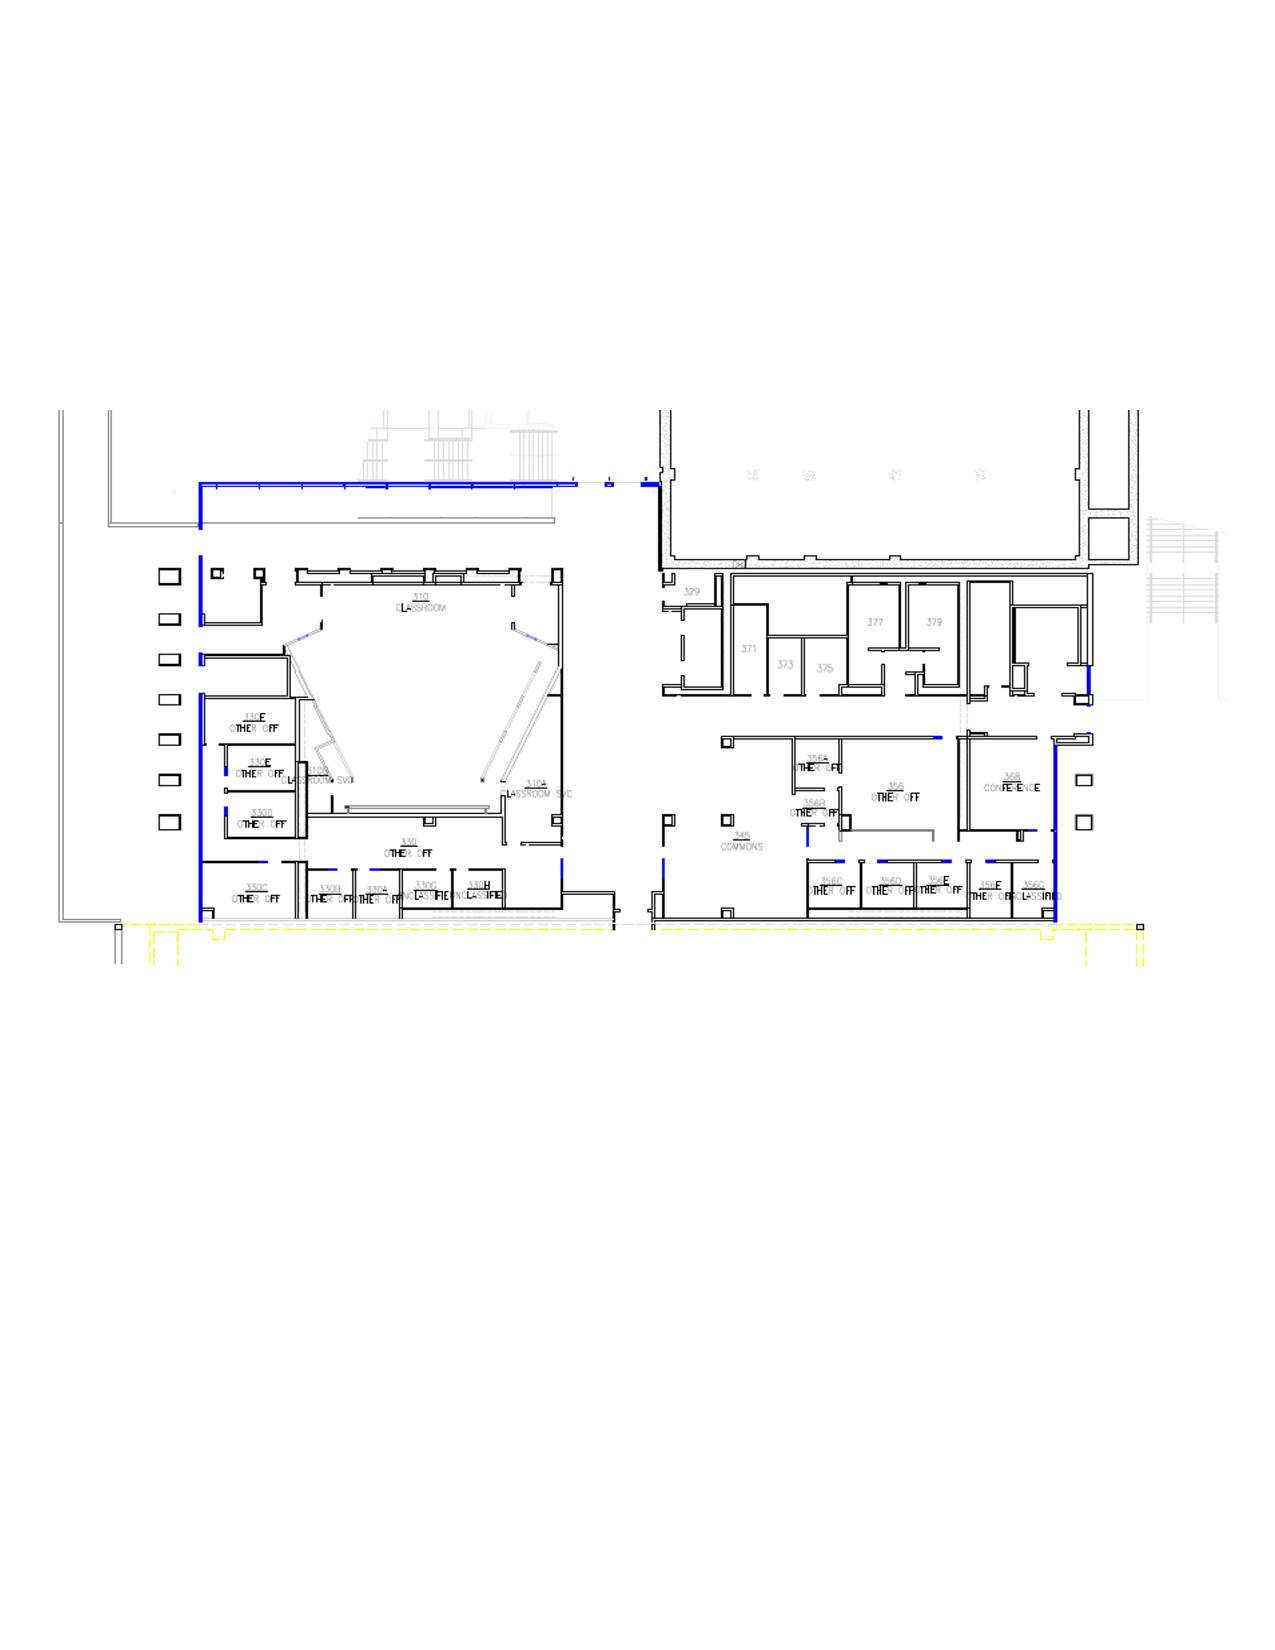
\includegraphics[width=0.4\textwidth]{./fig/SDH3_crop}
\caption{We collect data from 15 sensors in 5 rooms sitting on 4 different floors. This is a map of a section of the 3rd floor
in Sutardja Dai Hall.}
\label{fig:sdh}
\end{figure}

We perform an empirical study on sensor data collected from 15 sensors across 5 rooms. 
Each room has three sensors: a temperature sensor, a $CO_{2}$ sensor,  and a humidity sensor. 
The data from these is reported to an  
sMAP~\cite{smap} archiver. The data set used comes from two separate deployments: one is a deployment~\cite{Jay} lasting 
over 6 months on several floors in Sutardja Dai Hall (SDH) at UC Berkeley, where one sensor box -- which contains a thermometer, a humidity sensor
 and a $CO_{2}$ sensor -- is placed in each room. The box reports data over 6LowPAN~\cite{6lowpan} to a sMAP archiver every 
 15 seconds. The other is a long-term deployment comprised of thousands of sensors in dozens of buildings on campus. 
 We choose the portion of the SDH data set where the sensor devices, accessible via BACnet~\cite{BACnet}, report data to the archiver every few minutes. 
 Due to intermittent data loss, we pick a time span without interruption, starting in January until mid-February, 2013, for evaluation.
